\documentclass[11pt, a4paper]{article}
\usepackage{parskip}
\usepackage{calc}
%\usepackage[utf8]{inputenc} % Umlaute moussen nicht maskiert werden
\usepackage{fontspec} % Umlaute im eps sind nicht zusammengesetzt
\usepackage{lmodern} % Vektor-Schriftart
%\usepackage{ngerman} % Deutsche Silbentrennung (texlive-german und texlive-hyphen-german)
\usepackage{polyglossia}
\setmainlanguage{german}
\usepackage{graphicx} % Einbinden von Grafiken / SVG-Dateien moussen zuvor als eps exportiert werden
\usepackage{url} % Four URLs in der Bibliographie
\usepackage{amstext} % Four nichtkursiven Text in Formeln
\usepackage{subcaption}
\usepackage{listings}
\lstset{literate=%
	{Ö}{{\"O}}1
	{Ä}{{\"A}}1
	{Ü}{{\"U}}1
	{ß}{{\ss}}1
	{ü}{{\"u}}1
	{ä}{{\"a}}1
	{ö}{{\"o}}1
	{~}{{\textasciitilde}}1
}
\usepackage{subcaption}
\usepackage[dvipsnames]{xcolor}
\lstset{
	numbers= left,
	language=C++,
	keywordstyle=\color{Blue},
	stringstyle=\color{Orange},
	commentstyle=\color{OliveGreen},
	breaklines=true,
	extendedchars=true,
	basicstyle=\footnotesize\ttfamily,
	tabsize=4,
	frame=single,
	rulecolor=\color{black},
	captionpos=b,
	morekeywords={Vector3, Matrix, Transform, Vector4, Vector6,  EulerAngleXYZVector, Position, Vector, Rotation}}
\lstset{literate={-}{{-\allowbreak}}{1} }

\usepackage[export]{adjustbox}

\usepackage{etoolbox}% http://ctan.org/pkg/etoolbox
\makeatletter
\patchcmd{\lst@GLI@}% <command>
{\def\lst@firstline{#1\relax}}% <search>
{\def\lst@firstline{#1\relax}\def\lst@firstnumber{#1\relax}}% <replace>
{\typeout{listings firstnumber=firstline}}% <success>
{\typeout{listings firstnumber not set}}% <failure>
\makeatother
\newcommand{\code}{\texttt}
\usepackage{textcomp}
\usepackage{gensymb}
\usepackage{float}
\usepackage{csquotes}
\usepackage{amsmath}
\usepackage{microtype}
\usepackage{tikz}
\usepackage{xcolor}
\usetikzlibrary{shapes}
\usetikzlibrary{graphs}
\usetikzlibrary{graphdrawing}
\usegdlibrary{trees}
\date{\today}
\hyphenation{Trans-for-ma-ti-ons-ma-t-ri-zen, Trans-for-ma-ti-ons-ma-t-rix,Ko-or-di-na-ten-sys-teme,Ko-or-di-na-ten-sys-tem}
\begin{document}
\begin{center}
{\Huge Hochschule Darmstadt} \\
\vspace{0.5cm}
Lehrveranstaltung: Simulation von Robotersystemen \\
Dozent: Prof. Dr. Thomas Horsch \\
Laboringenieur: Rudi Scheitler \\
Versuch: Pfadsuche im Konfigurationsraum\\
Datum: 24.6.2016 \\
\vfill
\renewcommand{\arraystretch}{2}
	\begin{tabular}{| l | l |}
	\hline
	Name & Matrikelnummer \\ \hline
	Fabian Alexander Wilms & 735162 \\ \hline
	\end{tabular} \\
\vspace{0.5cm}
Studiengang: Mechatronik \\
Abgabedatum: 24.6.2016 \\
\renewcommand{\arraystretch}{1}
\end{center}
\newpage
\tableofcontents
\newpage
Konfigurationsräume geben an, für welche Gelenkstellungen ein Roboter mit seiner Umgebung kollidiert. Dies kann nun zur Bahnplanung genutzt werden. Sind für Start- und Zielpose alle Gelenkstellungen bekannt, so können beide  Posen durch je einen Punkt im Konfigurationsraum dargestellt werden. Vom Startpunkt aus soll jetzt ein Pfad zum Zielpunkt gesucht werden, wobei Kollisionen zu vermeiden sind.

\section{Kollisionsfreie Bahnplanung im Konfigurationsraum (Breitensuche)}
Es sind die Konfigurationsräume des letzten Praktikums sowie ein neuer gegeben. Da die Konfigurationsräume durch Stichproben entstanden sind, sind diese räumlich diskret und können als Bitmaps gespeichert werden. Das heißt, dass die Information, ob der Roboter mit der Umgebung kollidiert oder nicht nur mit einer endlichen Auflösung bekannt ist.

Jeder Konfigurationsraum stellt nun einen Graphen dar. Ein Graph ist eine Struktur, die aus einzelnen Knoten besteht, die untereinander verbunden sind. Jeder Knoten steht für eine Gelenkstellung, d.h. einen Pixel. In Fall zweidimensionaler Konfigurationsräume hat jeder Knoten 8 direkte Nachbarn. Der zu implementierende Algorithmus zur Bestimmung eines Pfads zwischen Start- und Zielpunkt nennt sich Breitensuche.

Es folgt eine Beschreibung des Algorithmus:

Der Startknoten wird in einer Warteschlange gespeichert (Schritt 1) und als bearbeitet markiert (Schritt 2). Falls die Warteschlange nicht leer ist, wird der älteste Knoten in dieser ausgelesen und aus ihr gelöscht (Schritt 3). Ist dieser der Zielknoten ist der Algorithmus beendet (Schritt 4). Anschließend untersucht man dessen direkte, noch nicht bearbeitete Nachbarn: Sie werden zunächst als bearbeitet markiert und, wenn die zugehörige Gelenkstellung keine Kollision verursacht, werden die Koordinaten der ursprünglichen Zelle in der neuen Zelle gespeichert und diese in der Warteschlange eingereiht (Schritt 5). Als nächstes wird zu Schritt 3 gesprungen.

Die folgenden Abbildungen illustrieren, dass zunächst alle direkten Nachbarn des aktuell betrachteten Knotens durchsucht werden, bevor man in die Tiefe geht.

\begin{figure}[H]
	% Kommentar am Ende ist wichtig, sonst falsche Längenberechnung
	\hfill
\center
\begin{subfigure}{\textwidth/\real{4.1}}
	\center\scalebox{0.35}{\begin{tikzpicture}
		\fill[yellow](2,4) rectangle (3,5);
		\fill[black] (3,1) rectangle (6,2);
		\fill[black] (3,6) rectangle (6,7);
		\fill[black] (5,1) rectangle (6,7);
		\fill[yellow] (2,4) rectangle (3,5);
		\fill[violet] (7,4) rectangle (8,5);
		\draw[gray,very thin] (0,0) grid (8,8);
		\end{tikzpicture}}
\end{subfigure}
\begin{subfigure}{\textwidth/\real{4.1}}
	\center\scalebox{0.35}{\begin{tikzpicture}
		\fill[yellow](2,4) rectangle (3,5);
		\fill[black] (3,1) rectangle (6,2);
		\fill[black] (3,6) rectangle (6,7);
		\fill[black] (5,1) rectangle (6,7);
		\fill[cyan] (1,3) rectangle (4,6);
		\fill[NavyBlue] (2,4) rectangle (3,5);
		\fill[violet] (7,4) rectangle (8,5);
		\draw[gray,very thin] (0,0) grid (8,8);
		\end{tikzpicture}}
\end{subfigure}
\begin{subfigure}{\textwidth/\real{4.1}}
	\center\scalebox{0.35}{\begin{tikzpicture}
		\fill[yellow](2,4) rectangle (3,5);
		\fill[cyan] (0,2) rectangle (5,7);
		\fill[NavyBlue] (1,3) rectangle (4,6);
		\fill[MidnightBlue] (2,4) rectangle (3,5);
		\fill[black] (3,1) rectangle (6,2);
		\fill[black] (3,6) rectangle (6,7);
		\fill[black] (5,1) rectangle (6,7);
		\fill[violet] (7,4) rectangle (8,5);
		\draw[gray,very thin] (0,0) grid (8,8);
		\end{tikzpicture}}
\end{subfigure}
\hfill %
	\caption{Konfigurationsraum: Die ersten drei Schritte einer BFS}
\end{figure}

\begin{figure}[H]
	% Kommentar am Ende ist wichtig, sonst falsche Längenberechnung
		\begin{subfigure}{\textwidth/\real{4.1}}
		\center\scalebox{0.7}{\begin{tikzpicture}[tree layout]\graph[nodes={draw, circle}] {
				a[fill,black,text=white,font=\bfseries] -> 
				{ 
					b -> 
					{ d, e ->
						h},
					c -> 
					{ f, g }
				}
			};
			\end{tikzpicture}}
	\end{subfigure}
	\begin{subfigure}{\textwidth/\real{4.1}}
		\center\scalebox{0.7}{\begin{tikzpicture}[tree layout]\graph[nodes={draw, circle}] {
				a[fill,black,text=white,font=\bfseries] -> 
				{ 
					b[fill,black,text=white,font=\bfseries] -> 
					{ d, e ->
						h},
					c[fill,black,text=white,font=\bfseries] -> 
					{ f, g }
				}
			};
			\end{tikzpicture}}
	\end{subfigure}
	\begin{subfigure}{\textwidth/\real{4.1}}
		\center\scalebox{0.7}{\begin{tikzpicture}[tree layout]\graph[nodes={draw, circle}] {
				a[fill,black,text=white,font=\bfseries] -> 
				{ 
					b[fill,black,text=white,font=\bfseries] -> 
					{ d[fill,black,text=white,font=\bfseries], e[fill,black,text=white,font=\bfseries] ->
						h},
					c[fill,black,text=white,font=\bfseries] -> 
					{ f[fill,black,text=white,font=\bfseries], g[fill,black,text=white,font=\bfseries] }
				}
			};
			\end{tikzpicture}}
	\end{subfigure}
	\begin{subfigure}{\textwidth/\real{4.1}}
		\center\scalebox{0.7}{\begin{tikzpicture}[tree layout]\graph[nodes={draw, circle}] {
				a[fill,black,text=white,font=\bfseries] -> 
				{ 
					b[fill,black,text=white,font=\bfseries] -> 
					{ d[fill,black,text=white,font=\bfseries], e[fill,black,text=white,font=\bfseries] ->
						h[fill,black,text=white,font=\bfseries]},
					c[fill,black,text=white,font=\bfseries] -> 
					{ f[fill,black,text=white,font=\bfseries], g[fill,black,text=white,font=\bfseries] }
				}
			};
			\end{tikzpicture}}
	\end{subfigure}%
	\caption{Graph: Die ersten vier Schritte einer anderen BFS}
\end{figure}

Implementiert wird die Breitensuche wie folgt:

Zu Beginn des Programms wird eine Bitmap-Datei eingelesen und im 2D-Array \code{char **cspace} gespeichert. Höhe und Breite der Datei werden ebenfalls gespeichert und verwendet, um ein weiteres 2D-Array zu erzeugen, diesmal vom Typ \code{Cell}. \code{Cell} ist ein \code{struct} und enthält folgende Elemente: \code{bool bMarked}, \code{int  nLastX} und \code{int  nLastY}.

Die Breitensuche findet in der Funktion \code{FindPath()} statt, der die Koordinaten des Start- und Zielpunktes übergeben werden. Diese Koordinaten beziehen sich auf das Koordinatensystem der Bitmap und nicht direkt auf die Gelenkvariablen.

Der erste Schritt  ist es, die einzelnen Zellen des Konfigurationsraumes zu initialisieren. Mit dem Wert des Elements \code{bMarked} wird angegeben, ob eine Zelle schon besucht wurde. Zunächst werden alle Zellen auf \code{bMarked = false} gesetzt werden.

Um bei der anschließenden Bestimmung des Pfads in \code{main()} nicht für jede Zelle entlang des Pfads überprüfen zu müssen, ob X- und Y-Koordinate schon mit den Sollwerten übereinstimmen, wird \code{nLastX} der Startzelle auf -1 gesetzt. Somit muss nur jeweils 1 Wert abgefragt werden.

Dann wird die Startzelle in die Queue eingefügt (Schritt 1) und markiert (Schritt 2). Die erste Zelle in der Queue wird ausgelesen und aus der Queue gelöscht. Solange noch Elemente in der Queue sind, wird nun eine \code{while}-Schleife ausgeführt (Schritt 3). Ist die Zelle die Zielzelle, so wird die Funktion beendet (Schritt 4). Dann folgt eine Schleife, welche achtmal läuft, einmal für jede Zelle, die potentiell an die aktuelle grenzt. Im Array \code{DirTable} stehen die relativen X- und Y-Koordinaten der Nachbarn, bezogen auf die aktuelle Zelle. Bei jedem der acht Schleifendurchläufe werden die relativen Koordinaten zu den absoluten aktuellen addiert (letztere sind für alle 8 Durchläufe gleich). Wurde die Zelle mit diesen neuen Koordinaten schon zuvor bearbeitet (\code{bMarked == 1}), so wird sie übersprungen. Andernfalls wird sie auf diese Art markiert und überprüft, ob die dazugehörige Gelenkstellung eine Kollision verursacht. Falls nicht, werden in der Zelle die vorherigen Koordinaten gespeichert (dies wird zur Rückverfolgung des Pfades benötigt) und die Zelle in der Warteschlange gespeichert (Schritt 5). Aufgrund der \code{while}-Schleife wird nun automatisch zu Schritt 3 gesprungen.

\begin{figure}[H]
	\center
	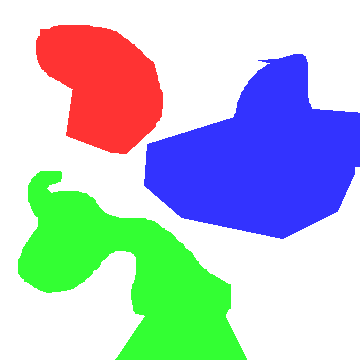
\includegraphics[width=0.4\textwidth,frame]{../Termin6/Termin6/cspace.png}
	\caption{Beispiel-Konfigurationsraum}
\end{figure}

\lstinputlisting[firstline=144,lastline=248,caption={Bestimmung des Konfigurationsraumes}]{../Termin6/Termin6/main.cpp}

Bei der BFS in 8er-Nachbarschaft sind die abgesuchten Konfigurationen rechteckig angeordnet:

\begin{figure}[H]
	\center
	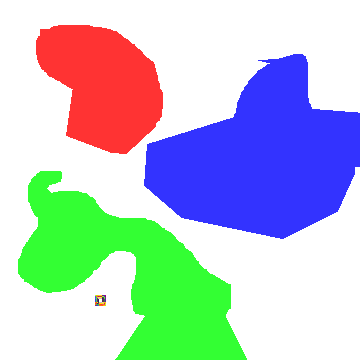
\includegraphics[width=0.5\textwidth,frame,viewport=75 35 125 85, clip]{../Termin6/Termin6/cspace_bfs_start.png}
	\caption{Beginn der Breitensuche (8er-Nachbarschaft)}
\end{figure}

Abgesuchte Konfigurationen sind im folgenden grün markiert:

Man sieht, dass ein -- wenn auch nicht optimaler -- Pfad gefunden wird:
\begin{figure}[H]
	\center
	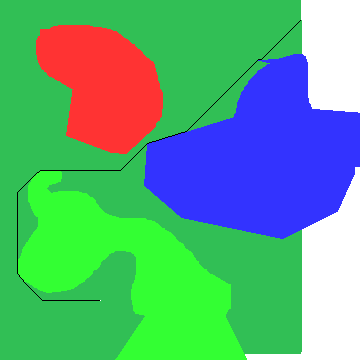
\includegraphics[width=0.5\textwidth,frame]{../Termin6/Termin6/cspace_bfs_8nb.png}
	\caption{Pfad im Beispiel-Konfigurationsraum (8er-Nachbarschaft)}
\end{figure}

Für den TT-Roboter ergibt sich folgender Pfad:

\begin{figure}[H]
	\center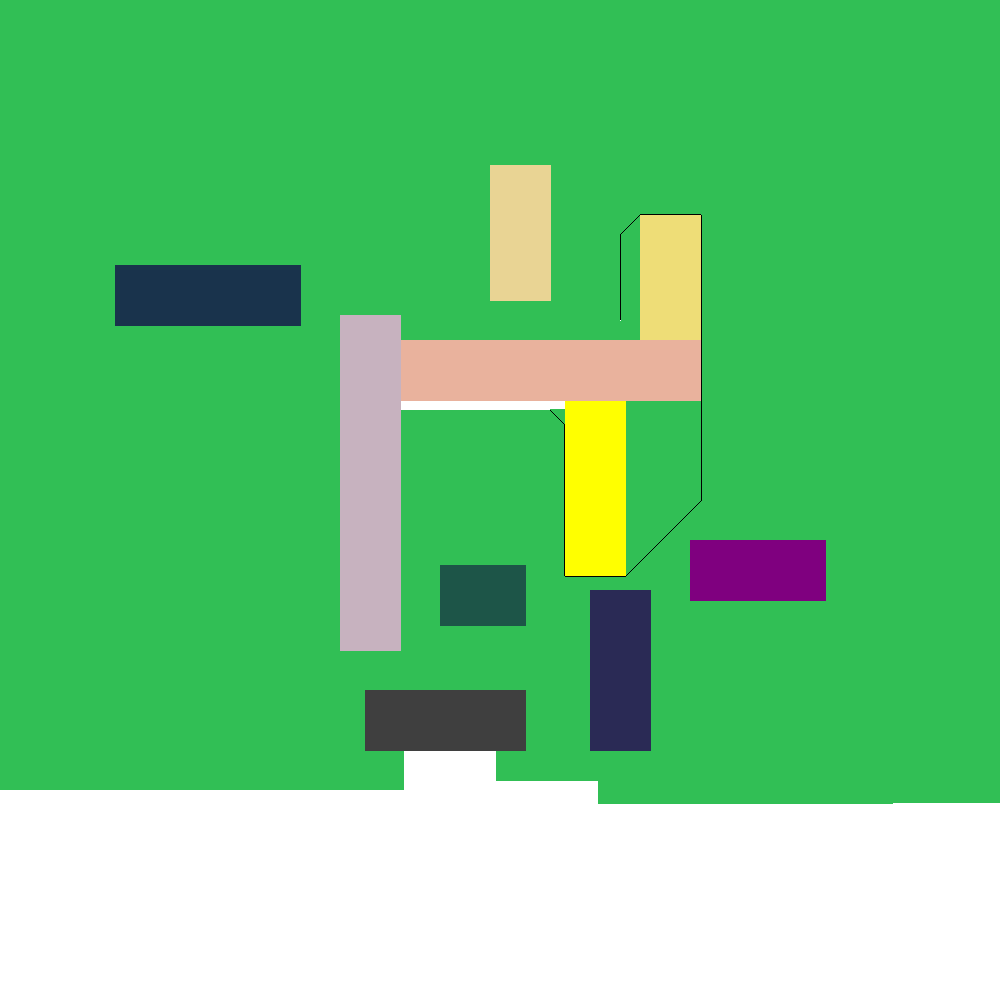
\includegraphics[width=0.5\textwidth,frame]{../Termin6/Termin6/cspace_prismatic_bfs.png}
	\caption{Bahn des TT-Roboters (8er-Nachbarschaft)}
\end{figure}

Führt man das erzeugte EasyRob-Programm mit aktiver TCP-Spur aus, so ergibt sich ein ähnliches Bild:

\begin{figure}[H]
	\center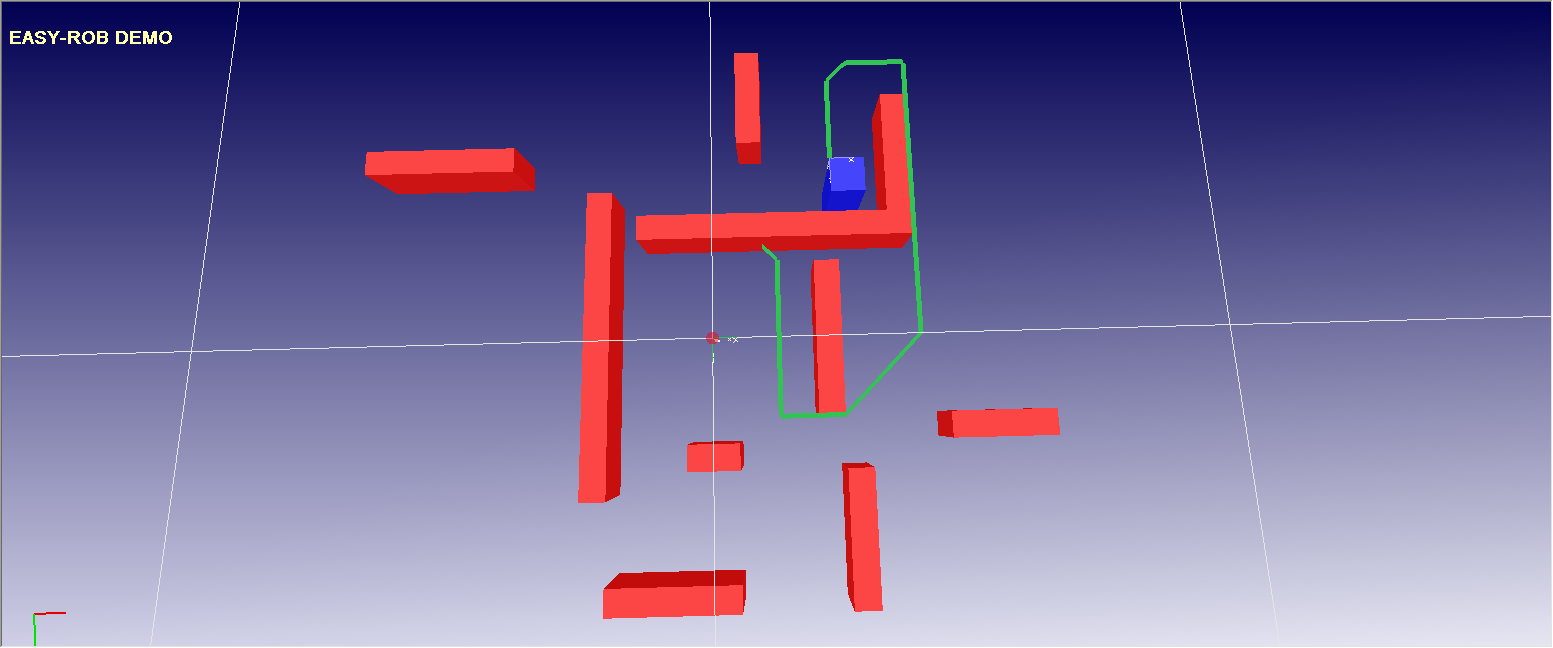
\includegraphics[width=0.75\textwidth]{prismatic.png}
	\caption{Bahn des RR-Roboters (8er-Nachbarschaft) in EasyRob}
\end{figure}

Zum Vergleich wird noch eine Pfadsuche in 4er-Nachbarschaft durchgeführt:

\begin{figure}[H]
	\center
	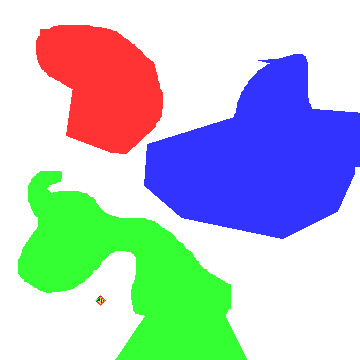
\includegraphics[width=0.5\textwidth,frame,viewport=75 35 125 85, clip]{../Termin6/Termin6/cspace_bfs_start_4nb.png}
	\caption{Beginn der Breitensuche (4er-Nachbarschaft)}
\end{figure}

Die abgesuchten Zellen sind in diesem Fall diamantförmig angeordnet

\begin{figure}[H]
	\center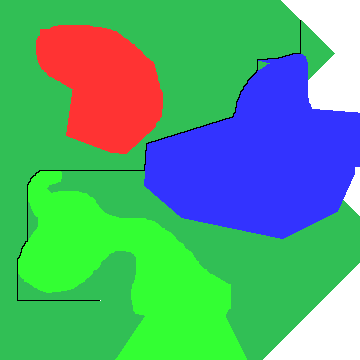
\includegraphics[width=0.5\textwidth,frame]{../Termin6/Termin6/cspace_bfs_4nb.png}
	\caption{Pfad im Beispiel-Konfigurationsraum (4er-Nachbarschaft)}
\end{figure}

Es fällt auf, dass bei der Suche in 4er-Nachbarschaft nur horizontale und vertikale Pfadstücke entstehen und bei der Suche in 8er-Nachbarschaft auch Strecken, die eine Rotation von \pm 45° haben.

Das bedeutet auch, dass eine 1 Pixel breite Diagonale nur bei der Suche in 8er-Nachbarschaft als Teil des Pfads in Frage kommt. Bei der Suche in 4er-Nachbarschaft wird bei folgendem Konfigurationsraum kein Pfad gefunden:

\begin{figure}[H]
	\center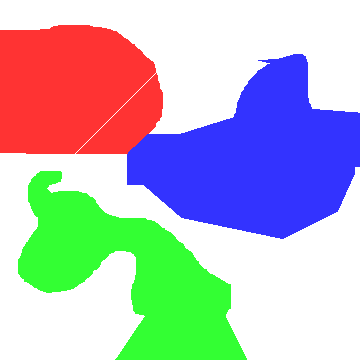
\includegraphics[width=0.5\textwidth,frame]{../Termin6/Termin6/cspace_1px.png}
	\caption{Modifizierter Beispiel-Konfigurationsraum;  Q\textsubscript{frei} enthält eine 45°-Diagonale}
\end{figure}

Bei der Suche in 8er-Nachbarschaft ist dies kein Problem:

\begin{figure}[H]
	\center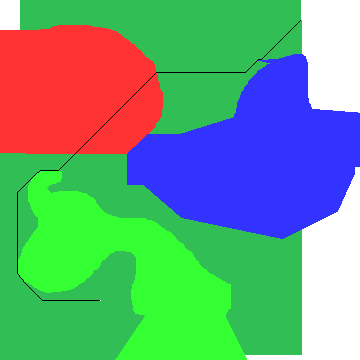
\includegraphics[width=0.5\textwidth,frame]{../Termin6/Termin6/cspace_1px_bfs_8nb.png}
	\caption{Pfad im modifizierten Beispiel-Konfigurationsraum  (8er-Nachbarschaft)}
\end{figure}

Die BFS funktioniert ohne Änderungen in \code{FindPath()} auch für RR-Roboter:

\begin{figure}[H]
	\center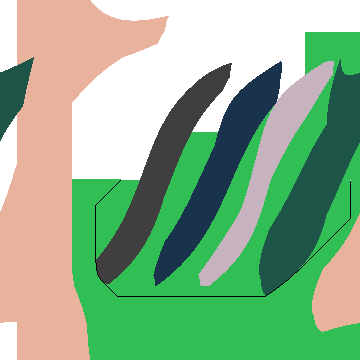
\includegraphics[width=0.5\textwidth,frame]{../Termin6/Termin6/cspace_revolute_bfs.png}
	\caption{Bahn des RR-Roboters (8er-Nachbarschaft)}
\end{figure}

Beim RR-Roboter fällt ein Vergleich der Bahn im Konfigurationsraum und in der Simulation schwerer. 
Markante Segmente des Pfads lassen sich dennoch wiedererkennen, wie zum Beispiel der Bereich, in dem q\textsubscript{2} konstant ist und sich nur q\textsubscript{1} ändert.

\begin{figure}[H]
	\center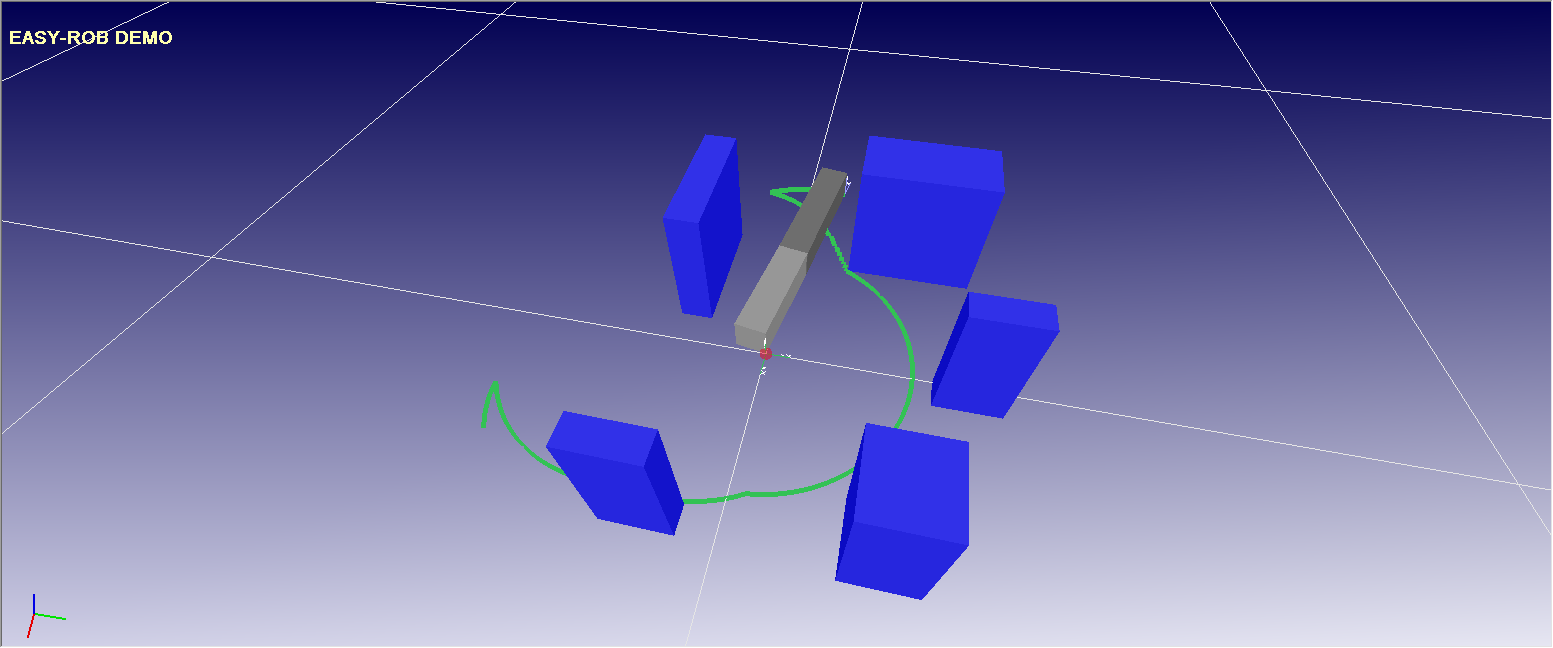
\includegraphics[width=0.75\textwidth]{revolute.png}
	\caption{Bahn des RR-Roboters (8er-Nachbarschaft) in EasyRob}
\end{figure}

Da zu Beginn eine andere Abfragereihenfolge der Nachbarkoordinaten vorgegeben war als die hier benutzte, konnte man feststellen, dass die Güte des gefundenen Pfades deutlich von dieser Reihenfolge abhängt. Insbesondere der ursprünglich gefundene Pfad für den RR-Roboter wich stark vom oben dargestellten ab.

\end{document}